% Created 2018-09-07 Fri 20:02
\documentclass[11pt]{article}
\usepackage[utf8]{inputenc}
\usepackage[T1]{fontenc}
\usepackage{fixltx2e}
\usepackage{graphicx}
\usepackage{grffile}
\usepackage{longtable}
\usepackage{wrapfig}
\usepackage{rotating}
\usepackage[normalem]{ulem}
\usepackage{amsmath}
\usepackage{textcomp}
\usepackage{amssymb}
\usepackage{capt-of}
\usepackage{hyperref}
\author{Eissa Nematollahi}
\date{2018-08-14}
\title{Being More Productive with Git\\\medskip
\large 20\% of Git you need to know to do 80\% percent of the work efficiently}
\hypersetup{
 pdfauthor={Eissa Nematollahi},
 pdftitle={Being More Productive with Git},
 pdfkeywords={},
 pdfsubject={},
 pdfcreator={Emacs 24.5.1 (Org mode 8.3.1)}, 
 pdflang={English}}
\begin{document}

\maketitle
\tableofcontents
\clearpage 
Git is the most popular \emph{Version Control System (VCS)} used by many software developers on projects of any scale. Most developers use Git on a daily basis, without having a deep understanding of how it actually works. You can significantly boost your productivity with a little more understanding of the Git workflow and how Git, as a distributed version control system, operates to manage repositories. My attempt, in this blog post, is to present minimal information you need to know to maximize your productivity with Git. For more detailed information, the reader may refer to Pro Git, which covers topics ranging from basic and intermediate levels, such as branching, merging, and rebasing, to advanced ones, such as rewriting history and working with submodules.

\section{History of Git}
\label{sec:orgheadline1}
Git was born out of frustration. The Linux development community had been using BitKeeper from 2002, however, its free license was revoked in 2005. The community decided to build a new version control system (VCS). Linus Torvalds, the creator of Linux, took initiative in this development. From the lessons learned over the three years of using BitKeeper, Linus was exactly aware of all the requirements and how to design a good VCS. The result was Git, which evolved over the years to be the most popular and most powerful VCS, employed in many projects of various scales across the world.

\section{Distributed vs. Centralized}
\label{sec:orgheadline2}
There are two types of version control systems: centralized and distributed. In a centralized system, like Subversion, changes are committed into a central repository on a remote server. Such a model has several drawbacks. First, the server may fail risking the whole repository. Therefore, a certain strategy must be developed for fault tolerance by means of redundancy, for example. Second, the server may temporarily be down, causing interruption among all users. Third, history of changes are only stored in a main remote repository. As a result, network connection is always required to check the history of commits.

In a Distributed VCS, like Git, each user has an exact copy of the remote repository. Such a model is fault tolerant, and every developer work mostly on a local copy of the repository offline. This model offers many other advantages. For example, modification can be split logically into separate commits. Once the work is completed, multiple commits can be pushed to one or more remote repositories. We do not need constant network connection to investigate the history of changes, since our local repository holds all the history of commits.

Git as a distributed VCS offers even more advantages. Branching is lightweight and merging is easy. This makes it possible to frequently diverge from the main branch, add a feature or fix bugs, and easily merge (or rebase) onto the main branch. Sometimes, we are in the middle of changes and not ready to stage or commit our changes, but we urgently need to fix a bug. Stashing is a great tool that stores changes temporarily, so we can fix the urgent bug first, and then apply the stash to our working directory and continue working.

\section{\label{orgtarget1} Setup}
\label{sec:orgheadline3}
To be more efficient with Git, I recommend using command-line tools with a proper setup to easily inspect the working directory and log history, check local and remote branches, and monitor modified, staged, or stashed files. In addition, using command-line tools, we can also fetch or pull updates from remote repositories, or push our updates to them.

User specific configurations are stored in the \texttt{\$HOME/.gitconfig} file. An example is given below:
\begin{verbatim}
# $HOME/.gitconfig file
[user]
  name = My Full Name
  email = myname@example.com
[core]
  editor = vim
[alias]
  lg = log --graph --decorate --oneline
  lga = log --graph --decorate --oneline --all
  st = status -s
  br = branch
  co = checkout
\end{verbatim}
The name and email address of the committer are set in this file, either directly or using \texttt{git config -{}-global} command as follows:
\begin{verbatim}
git config --global user.name "My Full Name"
\end{verbatim}
We can specify our editor of choice in this file, too. The editor will open when there is an automatic merge or when we use \texttt{git commit} command without providing a message. We can also define aliases for some git commands with options for convenience. In particular, \texttt{git log -{}-graph -{}-decorate -{}-oneline} and its many variations are useful when inspecting the log history and commits graph.

\section{Git Notations}
\label{sec:orgheadline6}
Git is a version control system that stores a series of coherent changes as a commit represented by a SHA-1 value, like \texttt{62840ed60259dca2bc90862672a663a9dcfe17b5}, whose abbreviated version \texttt{62840ed} is often used. When inspecting history of changes, we see a list of commits and connections among them to understand how a repository evolved over time.

Starting from the initial commit, we may diverge to multiple branches and merge later at some points in the future. Each commit may have one or two ancestors and multiple predecessors. Such relations among commits constitute a directed graph, which may look like Figure \ref{fig:orgparagraph1}.

\begin{figure}[htb]
\centering
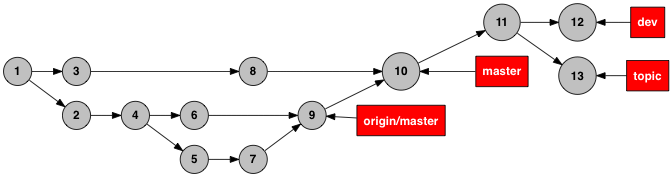
\includegraphics[width=.9\linewidth]{./images/commits-graph.png}
\caption{\label{fig:orgparagraph1}
Commits graph with 13 commit nodes and 3 local branches \texttt{master}, \texttt{dev}, and \texttt{topic} pointing to commits 10, 12, and 13, respectively, and one remote-tracking local branch \texttt{origin/master} pointing to commit 9.}
\end{figure}

Any commit can be referenced by its unique SHA-1 value. However, some commits may represent the tip of a branch and thus named like \texttt{master} or \texttt{origin/master}. Some commits may be labeled as a tag to indicate that the commit is a particular version like \texttt{v1.0.2}. There are also predefined names, like \texttt{HEAD}, \texttt{origin/HEAD}, \texttt{FETCH\_HEAD}, and symbols, like @, @\^{}, @\textasciitilde{}3, which are updated by Git to refer to special commits, like the current position. Note that pointers can move from one commit to another, but commits constitute history and (almost always) do not change.

\subsection{Ancestry References}
\label{sec:orgheadline4}
Notations \texttt{\textasciicircum{}} and \textasciitilde{} are used to point ancestors of a given commit. Each commit has only one parent except merge commits which have two parents. To access either parent of a merge commit, we use \texttt{\textasciicircum{}} notation. To access ancestors (parent of the parent of the parent, for example), use \textasciitilde{} notation. More details are given below:

\begin{enumerate}
\item \texttt{HEAD\textasciicircum{}} is equivalent to \texttt{HEAD\textasciicircum{}1} and means the first parent of \texttt{HEAD}. Merge commits have two parents: first parent, which is \texttt{HEAD}'s previous position, and the second parent, which is merged onto the other branch. The second parent can be addressed as \texttt{HEAD\textasciicircum{}2}. Note that \texttt{HEAD\textasciicircum{}3} does not have any meaning, since a commit cannot have more than two parents.
\item \texttt{HEAD\textasciitilde{}} is equivalent to \texttt{HEAD\textasciitilde{}1} and means the first parent of \texttt{HEAD}. Thus, \texttt{HEAD\textasciicircum{}} and \texttt{HEAD\textasciitilde{}} are equivalent too. However, \texttt{HEAD\textasciitilde{}2} means the first parent of the first parent. \texttt{HEAD\textasciitilde{}5} is meaningful and similarly defined; it is also equivalent to \texttt{HEAD\textasciicircum{}\textasciicircum{}\textasciicircum{}\textasciicircum{}\textasciicircum{}}.
\end{enumerate}

The following examples illustrate how \texttt{\textasciicircum{}} and \textasciitilde{} notations can be used to access ancestors of a given commit in Figure \ref{fig:orgparagraph1}.

\begin{itemize}
\item \texttt{dev\textasciicircum{}} and \texttt{dev\textasciitilde{}} both point to commit 11. They both mean the first parent of \texttt{dev}. If the commit-id of \texttt{dev} is \texttt{62840ed}, then \texttt{62840ed\textasciicircum{}} can also be used instead of \texttt{dev\textasciicircum{}}.
\item \texttt{dev\textasciicircum{}2} is not meaningful, since \texttt{dev} is not a merge commit.
\item \texttt{master\textasciicircum{}1} points to commit 8, while \texttt{master\textasciicircum{}2} points to commit 9, as does \texttt{origin/master}.
\item \texttt{topic\textasciitilde{}3} points to commit 8, and \texttt{topic\textasciitilde{}2\textasciicircum{}2} points to commit 9.
\end{itemize}

\subsection{\label{orgtarget3} Commit Ranges}
\label{sec:orgheadline5}
Git provides space (\texttt{A B}), double-dot (\texttt{A..B}), and triple-dot (\texttt{A...B}) notations to specify a range of commits, or better put, a set of commits. Commit ranges are used in the \texttt{git log} and \texttt{git rev-list} contexts. Although used in \texttt{git diff}, they do not really mean ranges, as explained in Section \hyperref[orgtarget2]{Differences between Two Commits}.

\begin{itemize}
\item \texttt{git rev-list master dev} lists, in reverse order, all the commits on branches ending to both \texttt{master} and \texttt{dev} commits, as shown in Figure \ref{fig:orgparagraph2}. It is commutative, i.e., \texttt{git rev-list dev master} produces the same output. This is typically not a very interesting case.
\item \texttt{git rev-list master..dev} lists, in reverse order, all the commits from \texttt{C} to \texttt{dev}, where \texttt{C} is the common ancestor of \texttt{master} and \texttt{dev}, as shown in Figure \ref{fig:orgparagraph3}. Note that the list excludes \texttt{C} but includes \texttt{dev}. It is not commutative, i.e., \texttt{git rev-list dev master} produces a different output.
\item \texttt{git rev-list master...dev} lists, in reverse order, all the commits from \texttt{C} to \texttt{master} or \texttt{dev}, where \texttt{C} is the common ancestor of \texttt{master} and \texttt{dev}. Note that the list excludes \texttt{C} but includes \texttt{master} and \texttt{dev}, as shown in Figure \ref{fig:orgparagraph4}. It is commutative, i.e., \texttt{git rev-list dev...master} produces the same output.
\end{itemize}

The command \texttt{git log} uses the commits produced by the \texttt{git rev-list} command to show the history associated with those commits.

\begin{figure}[htb]
\centering
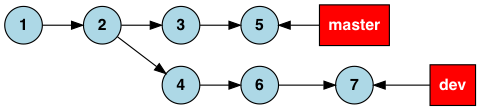
\includegraphics[width=.9\linewidth]{./images/commit-ranges-AB.png}
\caption{\label{fig:orgparagraph2}
Commits in blue are listed in the output of \texttt{git rev-list master dev} command.}
\end{figure}
\begin{figure}[htb]
\centering
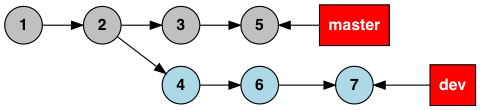
\includegraphics[width=.9\linewidth]{./images/commit-ranges-A__B.png}
\caption{\label{fig:orgparagraph3}
Commits in blue are listed in the output of \texttt{git rev-list master..dev} command.}
\end{figure}
\begin{figure}[htb]
\centering
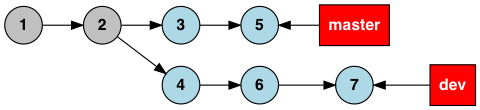
\includegraphics[width=.9\linewidth]{./images/commit-ranges-A___B.png}
\caption{\label{fig:orgparagraph4}
Commits in blue are listed in the output of \texttt{git rev-list master...dev} command.}
\end{figure}

\section{Git Workflow}
\label{sec:orgheadline7}
In this section, we will review the basics of the Git workflow. To better understand how Git actually works, it is important to know the following entities:
\begin{description}
\item[{Remote Repository}] Users clone from this repository and push their changes so others can retrieve and integrate with their changes. For example, \href{https://github.com/golang/go.git}{\url{https://github.com/golang/go.git}} is a remote repository which is publicly available for downloading. A remote repository can be just a bare repository, meaning that it may not contain a working directory, but does hold enough information to generate one.
\item[{Local Repository}] After cloning, users have a full copy of the remote repository where they can inspect history of commits, make changes, commit and push them into the remote repository. All the repository information is downloaded into the \texttt{.git} directory. When changes are committed, the local repository is updated. However, the remote repository is still not affected unless the committed changes are pushed.
\item[{Working Directory}] When cloning a repository, we get a full working directory beside the \texttt{.git} directory inside it. Every time we fetch from remote, we update the local repository, but the working directory is untouched. However, when we pull data from remote, we update both the local repository and the working directory. We will see that pulling means fetching and merging.
\end{description}
The diagram in Figure \ref{fig:orgparagraph5} shows an overview of the most common interactions among above three entities. In Table \ref{tab:orgtable1}, Git commands associated with all the actions are listed. More details about Git commands are provided in Section \hyperref[orgtarget4]{Git Basic Commands}.

\begin{figure}[htb]
\centering
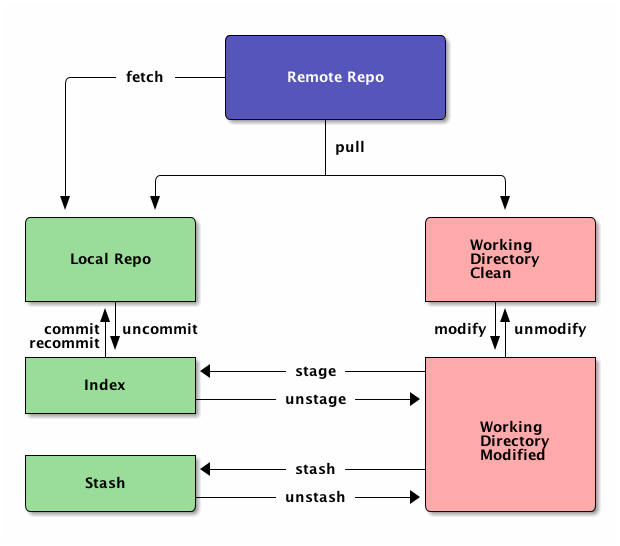
\includegraphics[width=.9\linewidth]{./images/git-workflow.png}
\caption{\label{fig:orgparagraph5}
Git workflow: interactions among working directory, local and remote repositories.}
\end{figure}

\begin{table}[htb]
\caption{\label{tab:orgtable1}
Git commands of the actions in Figure \ref{fig:orgparagraph5}. Note that the ``modify'' action includes addition, deletion, or any changes to files and folders in the working directory.}
\centering
\begin{tabular}{lll}
Action & Git command (Example) & Description\\
\hline
fetch & \texttt{git fetch origin master} & \\
pull & \texttt{git pull origin master} & fetch then merge\\
 & \texttt{git pull -{}-rebase origin master} & fetch then rebase\\
commit & \texttt{git commit -m"description of this commit"} & \\
recommit & \texttt{git commit -{}-amend} & modify last commit\\
uncommit & \texttt{git reset -{}-soft HEAD} & \\
stage & \texttt{git add -A} & \\
 & \texttt{git stage -A} & \\
unstage & \texttt{git reset HEAD} & \\
stash & \texttt{git stash} & \\
unstash & \texttt{git stash pop} & remove stash record\\
 & \texttt{git stash apply} & keep stash record\\
unmodify & \texttt{git reset -{}-hard HEAD; git clean -df} & changes lost\\
 & \texttt{git checkout -{}- .; git clean -df} & changes lost\\
\end{tabular}
\end{table}

\section{\label{orgtarget4} Git Basic Commands}
\label{sec:orgheadline20}
In this section, we will review the most frequently used git commands in most common situations.
\subsection{Create or Clone a Repository}
\label{sec:orgheadline8}
A local repository with a working directory may be cloned from a remote repository or created from scratch. To clone the Go language repository, for example, we simply run:
\begin{verbatim}
git clone https://github.com/golang/go.git
\end{verbatim}
To start a new project, we may create a repository in GitHub (or any similar host) first. GitHub typically provides instructions on how to setup a local directory for the repository, similar to the code below. First, navigate to the directory and create files with contents. Then, run the following commands to add and commit changes, create a link to the remote repository and push the commits.
\begin{verbatim}
git init
# make changes in this directory
git add -A
git commit -m "first commit"
git remote add origin https://github.com/myaccount/myrepo.git
git push -u origin master
\end{verbatim}
Some of these commands will be discussed in more details later. For now, it suffices to know that \texttt{git init} initializes the current directory as a Git repository by creating \texttt{.git} directory, where Git stores all its internal data. It automatically creates a branch called \texttt{master}. The command \texttt{git add} stages all the changes made in the local directory and \texttt{git commit} commits the staged changes into the local repository. Then, we create a remote reference called \texttt{origin} using \texttt{git remote add} command. Finally, we push the changes in our local \texttt{master} branch to the remote \texttt{master} branch using \texttt{git push} command.

A Git repository, whether local or remote, keeps all its data in the \texttt{.git} directory. Repository-specific configurations are stored in \texttt{.git/config} file. We can copy \texttt{.git} directory anywhere, and the folder containing it become a git repository. We can even clone it like \texttt{git clone \textasciitilde{}/myrepo/.git} somewhere to duplicate the repository. Although may not be useful, they verify that all the repository information are stored in the \texttt{.git} directory.

\subsection{\label{orgtarget5} Four States of a Local Repository}
\label{sec:orgheadline10}
In Git workflow, we are in one the following states:
\begin{enumerate}
\item The local repository is up-to-date and identical to the remote one, and the working directory is clean.
\item Working directory is modified, but changes have not yet been staged.
\item Changes are staged, but have not yet been committed.
\item Changes are committed, but have not yet been pushed to a remote repository
\end{enumerate}
Once the local changes are pushed to a remote repository in State 4, we return back to the State 1.

Suppose that we cloned a repository a while ago. Before making any changes, we use \texttt{git pull} command to make sure it has the latest commits. We are now at State 1.

Once we start making changes on the working directory, we transition from State 1 to State 2. We can inspect changes using \texttt{git status -s} command and the result may look like:
\begin{verbatim}
$ git status -s
 M README.md
?? test.go
\end{verbatim}
The inspection shows that the file \texttt{README.md} is modified but not staged, while \texttt{test.go} is not yet in the repository. To see more details of the changes in the files, we can run \texttt{git diff} as follows to see where in the files are modified.
\begin{verbatim}
$ git diff
diff --git a/README.md b/README.md
index 83c831f..89e7b14 100644
--- a/README.md
+++ b/README.md
@@ -1 +1,2 @@
 # test
+test.go implements a test program
\end{verbatim}
As it can be seen, we added a line in the \texttt{README.md} file.

To undo the changes, we can run either \texttt{git reset -{}-hard HEAD} or \texttt{git checkout -{}- .} command. Note that untracked files may be in the working directory, which can manually be removed using Linux's \texttt{rm} command or Git's \texttt{git clean -df} command. These commands are dangerous as they wipe out all the changes which are not saved in the history of the Git repository. As a word of caution, make sure to run \texttt{git clean -dfn} command first for a dry-run to list all the files that are going to be deleted.

Once we complete our changes, we need to stage them using \texttt{git add} command and transition from State 2 to State 3. Note that the sub-command \texttt{add} for staging is a bit misleading. That is why there is an alias for it: \texttt{git stage}, as you may have guessed. We can stage modified files one by one, or use option \texttt{-A} to stage all the changes. As before, we can check the status using \texttt{git status -s} command.
\begin{verbatim}
$ git status -s
M  README.md
A  test.go
\end{verbatim}
The inspection shows that the file \texttt{README.md} is modified and staged, and \texttt{test.go} is newly added and staged. After changes are staged, \texttt{git diff} will not show anything. To see the details of file changes after staging, we should use \texttt{git diff -{}-cached} command. To see all the staged and unstaged changes, we can run \texttt{git diff HEAD} command. For more use-cases of the \texttt{git diff} command, refer to Section \hyperref[orgtarget2]{Differences between Two Commits}.

To unstage changes, we can use \texttt{git reset HEAD}. As we will see later, \texttt{reset} is a useful sub-command, but caution must be taken when using it, as it may erase all the changes.

After changes are staged, we can commit them using \texttt{git commit} command. It's often followed by \texttt{-m} option to provide a message as string, explaining what changes the commit includes. Once the changes are committed, the status will be clean and \texttt{git status -s} will return nothing.

To undo the last commit, we can run \texttt{git reset -{}-soft HEAD\textasciitilde{}} command. As you may have guessed, the command \texttt{git reset HEAD\textasciitilde{}} undoes both the commit and staging the changes.

After committing and before pushing, we may realize that we have forgotten some changes. In such a situation, we can easily amend our changes to the last commit using \texttt{git commit -{}-amend} command. We will be prompted to update the commit message in an editor, like Vim. Once we save and exit the editor, the changes will be applied. If we do not wish to update the commit message, we can run \texttt{git commit -{}-amend -{}-no-edit} command.

\subsubsection{Summary}
\label{sec:orgheadline9}
In summary, we have four states for a local repository and can move between states as follows:
\begin{itemize}
\item Start coding and modify the repository as you wish.
\item Stage changes using \texttt{git add} or \texttt{git stage} command.
\item Commit staged changes using \texttt{git commit} command.
\item Push committed changes to a remote repository using \texttt{git push} command and return to a clean working directory.
\end{itemize}

To undo above changes, we mainly use the dangerous-looking \texttt{git reset} command as follows:
\begin{itemize}
\item To undo the last commit and move to the staged state, run \texttt{git reset -{}-soft HEAD\textasciitilde{}}
\item To redo the last commit by amendment, run \texttt{git commit -{}-amend -{}-no-edit}
\item To undo the staged changes and move to the modified state, run \texttt{git reset HEAD}
\item To undo the modification and move to the clean state, run \texttt{git reset -{}-hard HEAD}. We may need to run \texttt{git clean -df} to clean up the untracked files and directories.
\end{itemize}

To inspect changes in the local repository, we can use the following commands:
\begin{itemize}
\item Run \texttt{git status -s} to obtain a short status of the modified or staged files.
\item Run \texttt{git diff} to see more details of the file changes before they are staged.
\item Run \texttt{git diff -{}-cached} to see more details of the file changes after they are staged.
\end{itemize}

\subsection{Branching}
\label{sec:orgheadline11}
Branching mechanism is one of the best features of Git. It is so lightweight, fast, and efficient that is used on a daily basis. Branching is used to temporarily diverge from the main branch, like \texttt{master}, to fix bugs or add new features in a new branch, like \texttt{dev}. The new branch, containing all the local changes, is integrated with the main local branch by merging or rebasing, which is discussed in more details in Section \hyperref[orgtarget6]{Rebase vs. Merge}.

In this section, we will discuss branch types and how to create, delete, and inspect branches. We will also review the most frequently used git commands related to branching.

There are three types of branches:
\begin{enumerate}
\item Local branches, like \texttt{master}.
\item Local remote-tracking branches, like \texttt{origin/master}.
\item Remote branches, like \texttt{remotes/origin/master}.
\end{enumerate}

To see all the local and remote branches, use \texttt{git branch -a} command. A typical output may look like:
\begin{verbatim}
$ git branch -a
  bug-fix
  dev
* master
  remotes/origin/HEAD -> origin/master
  remotes/origin/master
  remotes/origin/dev
\end{verbatim}
As the output shows, there are three local branches (\texttt{bug-fix}, \texttt{dev}, and \texttt{master}), with \texttt{master} being the currently checked-out branch. In addition, there are two remote branches (\texttt{dev} and \texttt{master}). We will focus on working with local branches here and discuss remote branches in Section \hyperref[orgtarget7]{Remote Repository}. To list remote-tracking branches associated with certain branches, run \texttt{git branch -vv} command.

We can switch between local branches using \texttt{git checkout} command. For example, to switch to the \texttt{dev} branch from the \texttt{master} branch, we run \texttt{git checkout dev} command.

To check out a remote branch, however, we can create a local branch to track the remote one. Suppose that we need to review the changes of a colleague on a different remote branch. We can checkout the remote branch as a new local branch as follows:
\begin{verbatim}
git checkout -b review-steve origin/steve
\end{verbatim}
This command creates a new local branch \texttt{review-steve}, which points to the remote-tracking branch \texttt{origin/steve}, and switches to it.

Suppose that the \texttt{master} branch is up-to-date, and we would like to add a new feature to our project. A typical workflow is to create a new branch, temporarily diverge from the \texttt{master} branch, commit changes, and apply (merge or rebase) changes to the \texttt{master} branch. To create a new branch \texttt{feature} and switch to it, we use \texttt{git checkout -b feature} command.

To delete a local branch, use \texttt{git branch -d dev} command. This fails if the \texttt{dev} branch is not yet merged, since all the commits on this branch would be lost. Such branches can be forced to be deleted using \texttt{git branch -D dev} command.

Deleting a local branch does not affect its associated remote-tracking branch. For example, suppose that \texttt{origin/dev} is a remote-tracking branch associated with \texttt{dev}. To delete a remote-tracking branch, run \texttt{git branch -d -r origin/dev} command. Note that deleting a remote-tracking local branch does not affect the remote branch. We will see in Section \hyperref[orgtarget7]{Remote Repository} how to delete a remote branch.

\subsection{\label{orgtarget6} Rebase vs. Merge}
\label{sec:orgheadline12}
Rebasing and merging are two different approaches to converge from one branch to another and integrate them. Suppose that we diverged from the \texttt{master} branch by creating a new branch \texttt{dev} and adding a few commits. Before updating \texttt{master} with our changes in the \texttt{dev} branch, we run \texttt{git fetch} to make sure the \texttt{master} branch is not behind its remote counterpart.

To integrate our changes, we can switch to the \texttt{master} branch, and run \texttt{git merge dev} command. There might be conflicts that should be resolved, which will be discussed in more details in Section \hyperref[orgtarget8]{Resolving Conflicts}. Merging often results in adding a merge commit that shows where two branches are converged, unless it is fast forwarded. Note that fast-forwarding happens only if \texttt{dev} branch is on the same line but ahead the \texttt{master} branch.

Another way to integrate our changes is to rebase \texttt{dev} onto \texttt{master} which takes all the changes from \texttt{dev} and applies them on top of the \texttt{master} branch. This results in a neater history and is a preferred approach. To perform rebase, switch to the \texttt{dev} branch and run \texttt{git rebase master} command.

\textbf{NOTE:} Rebasing often results in a cleaner history of commits than merging. However, there is case that can have unpleasant consequences: rebasing remote branches onto another one and pushing the final commits rewrites the history. As a general rule, always use rebasing to rebase a local branch onto another local or remote branch.

In summary, we can integrate branches by merging or rebasing. We should prefer rebasing over merging as it results in a neater history of commits. However, bear in mind that only local branches should be rebased onto the remote-tracking branching and not the other way around. The following approaches are equivalent and preferred approaches:
\begin{itemize}
\item Run \texttt{git fetch} to update remote-tracking local branches. Then, run \texttt{git rebase origin/master} from the \texttt{master} branch to rebase \texttt{master} onto the \texttt{origin/master} and integrate them.
\item Run \texttt{git pull -{}-rebase origin master} to pull from the remote repository into the \texttt{master} branch with rebasing.
\end{itemize}

\subsection{Stashing}
\label{sec:orgheadline13}
Suppose that we are in the middle of some changes to our project. The build is broken so we do not want to commit the changes yet. However, we receive a message that we have to fix an issue urgently. We do not want to lose the changes, but we want to save it so that we can retrieve them after the bug is fixed. Stashing is a great tool in such a situation.

To stash current changes, run \texttt{git stash} command. Then, run \texttt{git stash list} to see the list of all changes that are stashed. A typical output of the latter command may look like:
\begin{verbatim}
$ git stash list
stash@{0}: On dev: division
stash@{1}: WIP on master: db2ac73 added add.go file
\end{verbatim}
The list shows that there are two stashed changes: one on the \texttt{dev} branch and another on the \texttt{master} branch. To inspect each stash point, run \texttt{git stash show stash@\{1\}} command.

After stashing, the working directory is clean and we can perform our urgent fix on the project, commit the changes, and push them. Then, run \texttt{git stash apply} to apply the last stashed change back to the working directory and continue coding. To apply a particular stash, we can run \texttt{git stash apply stash@\{1\}} command.

The stashed data will still be there, but can be removed using \texttt{git stash drop stash@\{1\}} command. If the stash reference is not specified, it drops the top stash, which is \texttt{stash@\{0\}}. The shortcut to apply and drop a particular stash is \texttt{git stash pop @stash\{2\}} command.

Note that newly added, modified, and staged files can be stashed. When retrieved, they will retain their previous states. Untracked files will not be stashed, though. To stash untracked files as well, run \texttt{git stash -u} command. To stash even ignored files as well, run \texttt{git stash -{}-all} command.

\subsection{\label{orgtarget7} Remote Repository}
\label{sec:orgheadline14}
To publish our local committed changes, we need to push them to a remote repository that is accessible to other users. In this section, we will learn how to work with one or more remote repositories. Git commands related to remote repositories and branches start with \texttt{git remote}.

To see all the remote repositories, run \texttt{git remote -v} command. A typical output with one remote may look like:
\begin{verbatim}
$ git remote -v
origin  https://github.com/eissana/test.git (fetch)
origin  https://github.com/eissana/test.git (push)
\end{verbatim}

To update a remote URL, use \texttt{git remote set-url} command. For example, to avoid being prompted to provide username when fetching, pulling, or pushing, we can update the URL as follows:
\begin{verbatim}
git remote set-url origin https://eissana@github.com/eissana/test.git
\end{verbatim}
We will still be prompted to provide password every time we want to access a remote repository. To simplify this, we can run \texttt{git config -{}-global credential.helper 'cache -{}-timeout=300'} to avoid password interruption for five minutes.

The reference name for the remote repository is \texttt{origin}, by default, but it can be renamed. To get more details about the \texttt{origin}, run \texttt{git remote show origin} command. The output of this command may look like:
\begin{verbatim}
$ git remote show origin
* remote origin
  Fetch URL: https://github.com/eissana/test.git
  Push  URL: https://github.com/eissana/test.git
  HEAD branch: master
  Remote branch:
    master tracked
  Local branch configured for 'git pull':
    master merges with remote master
  Local ref configured for 'git push':
    master pushes to master (up to date)
\end{verbatim}

As we have seen before, to list all local and remote branches, we can run \texttt{git branch -a} command. Suppose that we have a local branch \texttt{dev}. The first time we run \texttt{git push origin dev}, a remote branch \texttt{remotes/origin/dev} is created. Local \texttt{dev} branch is not tracked by the remote branch, unless we specify it when pushing to it for the first time as \texttt{git push -u origin dev}. In this case, a local remote-tracking branch \texttt{origin/dev} is created.

We have previously discussed how to delete a local and remote-tracking local branches. They do not affect the remote \texttt{remotes/origin/dev} branch. To actually delete the remote branch, run \texttt{git push origin -{}-delete dev} command.

It is possible and often useful to push changes from a local branch, like \texttt{dev}, to another remote branch, like \texttt{origin/master}, which does not track \texttt{dev}. This can be achieved by simply running \texttt{git push origin dev:master} command.

To get data from a remote repository, we may use either \texttt{git pull} or \texttt{git fetch} command. If the repository is clean and we have not made any changes or commits, then \texttt{git pull} is the simplest way to obtain and apply remote changes into our working directory. Otherwise, it might be a better idea to first fetch the changes without affecting our working directory, then use \texttt{git log} command to inspect the history of changes before applying them into the working directory.

The main difference between \texttt{git pull} and \texttt{git fetch} is that the latter fetches all the remote changes into the remote-tracking local branches, like \texttt{origin/master}, without affecting the working directory. However, the former downloads all the remote changes and applies them into the working directory. In fact, in a clean working directory, the effect of running \texttt{git fetch origin master} and then \texttt{git merge origin/master} from the \texttt{master} branch is the same as running \texttt{git pull origin master} command.

Performing \texttt{git fetch origin master} followed by \texttt{git rebase origin/master} results in a cleaner history. This is equivalent to \texttt{git pull -{}-rebase origin master} command.

\subsection{Inspecting History}
\label{sec:orgheadline17}
Main tools for commits history inspection include \texttt{git log} and \texttt{git reflog} commands. We have seen some variants of \texttt{git log} in Section \hyperref[orgtarget1]{Setup}. In this section, we will discuss more details on its useful options and how to obtain an overview of the log history to understand what has happened in the remote repository. In addition, we will also discuss ways to inspect the reference log history to trace back the tips of branches and in particular \texttt{HEAD}. This is very useful for finding lost commits.

For a file-level inspection, we can use \texttt{git blame} tool. For example, \texttt{git blame README.md} lists details of the changes on each line of the code, including the author. Thus, inspecting the file using \texttt{git blame} tool can reveal whom to blame for a faulty change in a certain file.

\subsubsection{Commits Log}
\label{sec:orgheadline15}
Managing multiple local and remote branches and multiple repositories in a collaborative environment can be challenging. That is why having a tool to visualize and summarize the history of changes in the repositories is of great importance. The plain \texttt{git log} command will show the list of the commits and its details. However, for better visualization we need to use its options. In particular \texttt{git log -{}-graph} shows the commits on different branches and how they are diverged from a common ancestor or how they merged. \texttt{git log -{}-graph -{}-decorate} labels the tip of local and remote-tracking branches. This is important in understanding where each branch is positioned relative to others. The result might be pretty crowded with many details like long commit messages. To simplify this and have a neat graph, we can use \texttt{git log -{}-graph -{}-decorate -{}-oneline} command. The top line will be the tip of the current branch. We often need to see the big picture with having all branches. In such a
case, we use \texttt{git log -{}-graph -{}-decorate -{}-oneline -{}-all} command. We can customize the graph to show one of more selected branches rather than showing all of them. For example, \texttt{git log -{}-graph -{}-decorate -{}-oneline master dev} will not show branches other than \texttt{dev} and \texttt{master} unless they are along these two branches.

We can format the output of the \texttt{git log} command using its \texttt{-{}-pretty} option. For example, The following command formats the commit history provided by the pretty option.
\begin{verbatim}
git log --graph --pretty=format:'%Cred%h%Creset -%C(yellow)%d%Creset %s %Cgreen(%cr) %C(bold blue)<%an>%Creset'
\end{verbatim}
Its output may look like as follows:

\begin{figure}[htb]
\centering
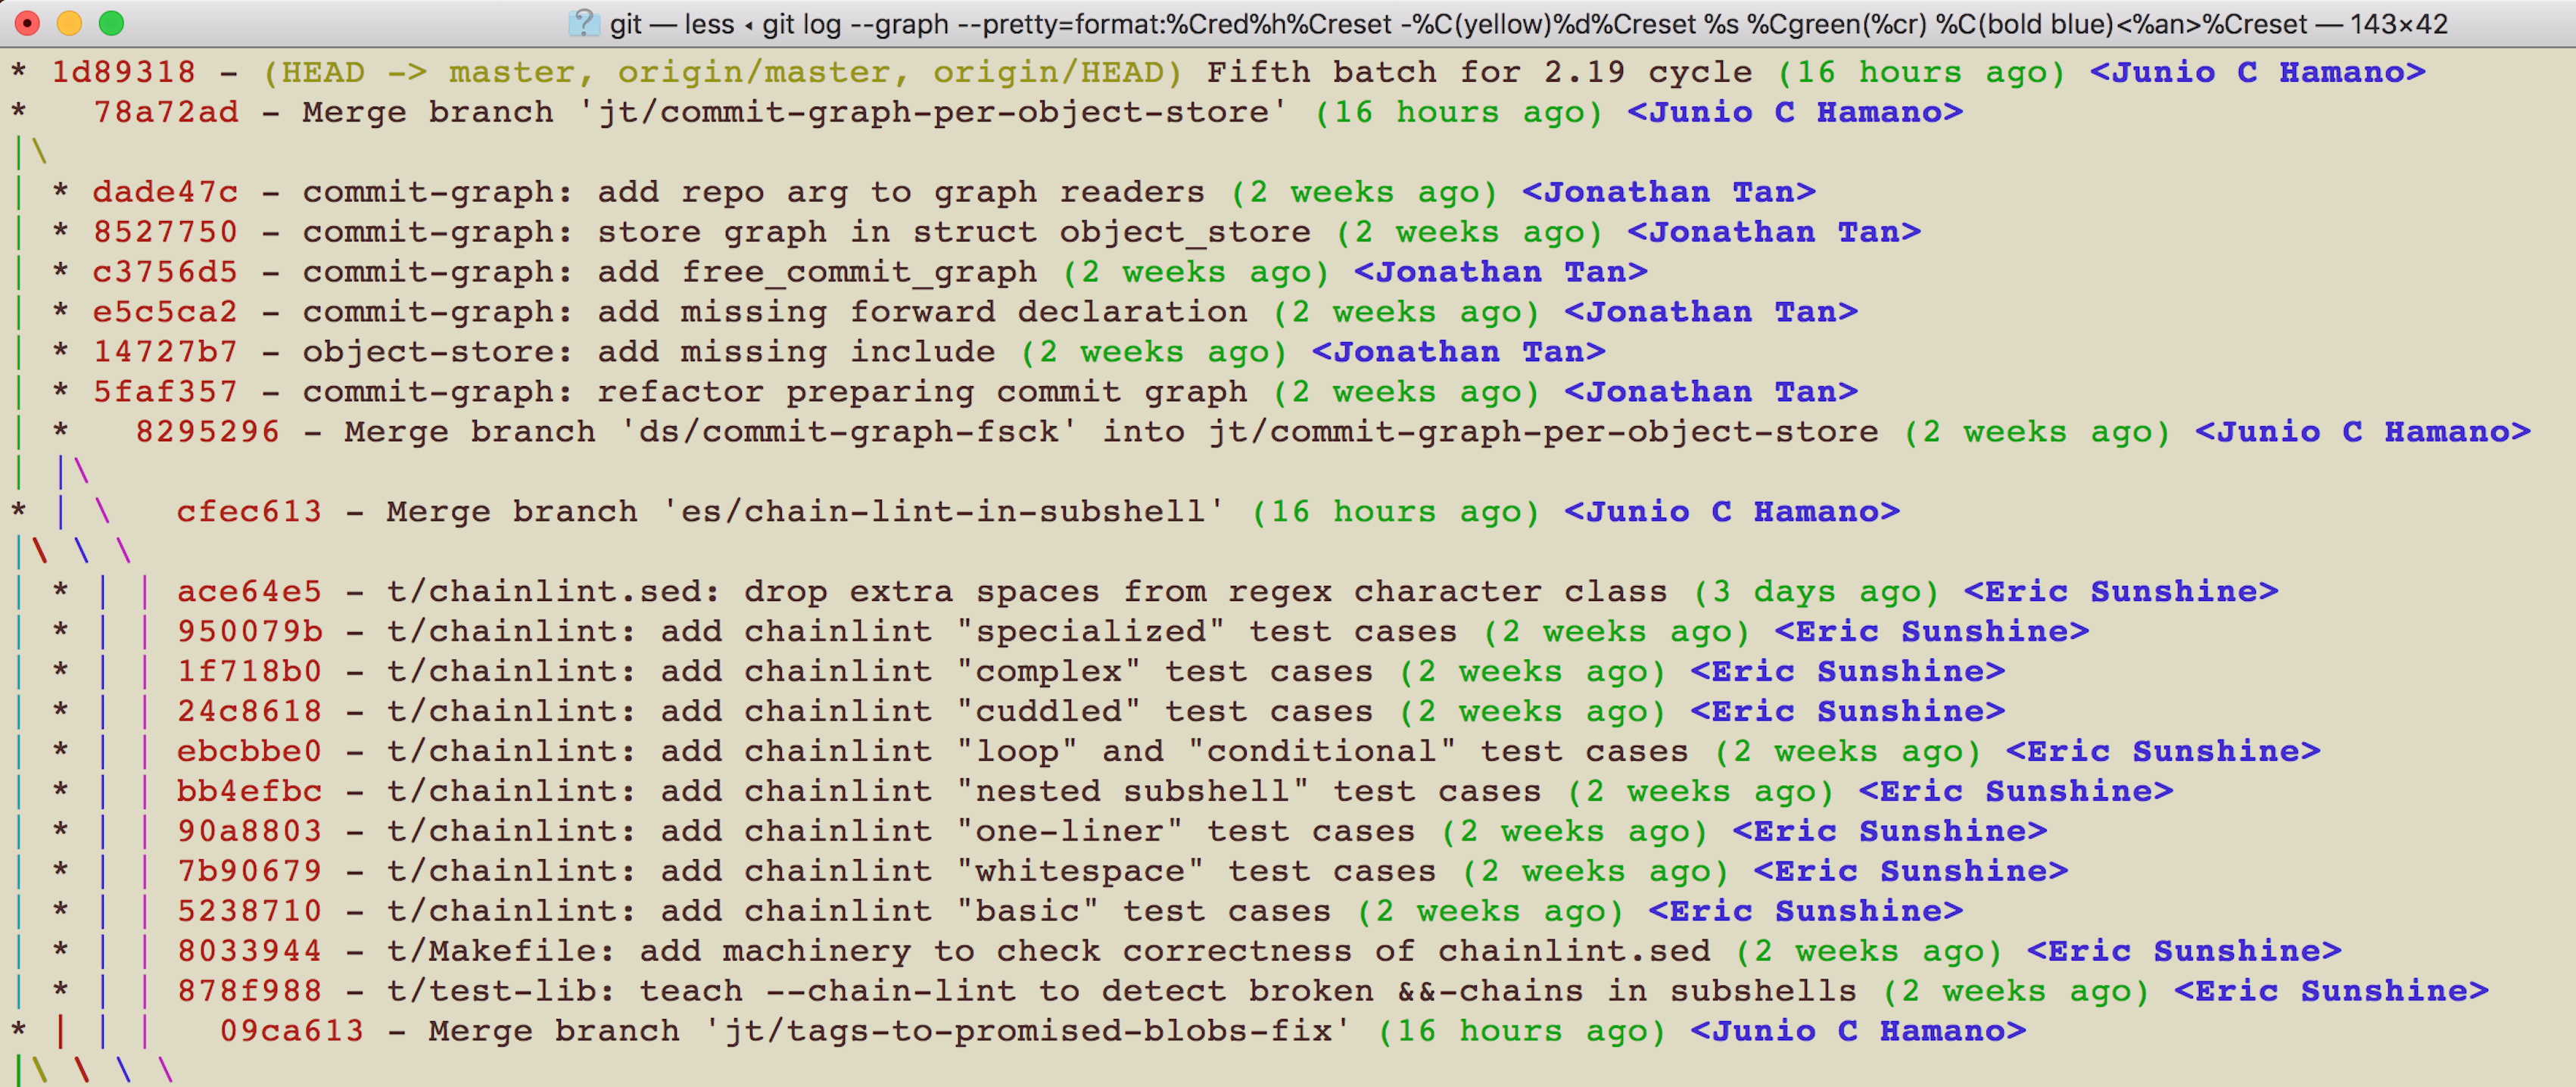
\includegraphics[width=.9\linewidth]{./images/git-log-pretty-1.png}
\caption{\label{fig:orgparagraph6}
An output of the \texttt{git log} command with pretty formatting.}
\end{figure}

To output only the last few commits, say 10, we can use \texttt{git log -10} command. Additionally, we can use \hyperref[orgtarget3]{Commit Ranges} to show the logs of certain commits in specified ranges.

\subsubsection{Reference Log}
\label{sec:orgheadline16}
Reference log command \texttt{git reflog} outputs the historical position of the \texttt{HEAD} or any local branch that is passed to it as an argument like \texttt{git reflog dev} command. The following output is an example of running \texttt{git reflog} command:
\begin{verbatim}
$ git reflog
5d9e28c HEAD@{0}: commit: Modified test file
8085ed2 HEAD@{1}: checkout: moving from master to dev
8085ed2 HEAD@{2}: commit: Created test file
1d89318 HEAD@{3}: clone: from https://github.com/git/git.git
\end{verbatim}
The reference log output shows the history of where \texttt{HEAD} has moved. First, we cloned a repository and committed some changes. Then, we switched from \texttt{master} branch to the \texttt{dev} branch and committed some other changes.

Reference log history is useful in recovery of lost commits. Here is a possible scenario. Suppose that we created a new branch \texttt{dev} as in the previous example. Then, we accidentally deleted the branch using \texttt{git branch -D dev} command. Now, the whole branch is removed. Git almost always adds data to the repository and only once in a while runs a garbage collector to clean unused objects. Thus, there must be a way to recover the lost branch. Running \texttt{git reflog -{}-decorate} yields the following output:
\begin{verbatim}
$ git reflog --decorate
 8085ed2 (HEAD -> master) HEAD@{0}: checkout: moving from dev to master
 5d9e28c HEAD@{1}: commit: Modified test file
 8085ed2 (HEAD -> master) HEAD@{2}: checkout: moving from master to dev
 8085ed2 (HEAD -> master) HEAD@{3}: commit: Created test file
 1d89318 (origin/master, origin/HEAD) HEAD@{4}: clone: from https://github.com/git/git.git
\end{verbatim}
Inspecting the output, we can easily find out that the tip of the removed \texttt{dev} branch was at \texttt{HEAD@\{1\}} position. To recover the lost branch, we run the following command:
\begin{verbatim}
git checkout -b dev HEAD@{1}
\end{verbatim}

\subsection{\label{orgtarget2} Differences between Two Commits}
\label{sec:orgheadline18}
The main tool to check the differences between two commits is \texttt{git diff} command. We have previously seen some of its use cases in Section \hyperref[orgtarget5]{Four States of a Local Repository}. In this section, we will see how to list all the changes introduced between two given commits.

Space, double-dot, and triple-dot notations are introduced in Section \hyperref[orgtarget3]{Commit Ranges}. As we noted there, it is a misconception to use commit ranges in \texttt{git diff} command, since double- and triple-dot notations in this context do not really mean a range of commits. We will see the reason shortly.

\begin{enumerate}
\item \texttt{git diff master dev} command means get all the changes between \texttt{master} and \texttt{dev}; see Figure \ref{fig:orgparagraph7}. It is not commutative, i.e, \texttt{git diff dev master} generates different output, which is the reverse of the output of \texttt{git diff master dev} command.
\item \texttt{git diff master..dev} command is equivalent to \texttt{git diff master dev} and there is no range of commits involved; see Figure \ref{fig:orgparagraph7}.
\item \texttt{git diff master...dev} command means get the difference between commit \texttt{C} and \texttt{dev}, where \texttt{C} is the common ancestor of \texttt{master} and \texttt{dev}; see Figure \ref{fig:orgparagraph8}. It is not commutative, this \texttt{git diff dev..master} generates different output.
\end{enumerate}

The common ancestor of \texttt{master} and \texttt{dev} can be obtained using \texttt{git merge-base master dev} command. We can verify that \texttt{git diff master...dev} is equivalent to \texttt{git diff \$(git merge-base master dev) dev} command.

As we observed, neither \texttt{A..B} nor \texttt{A...B}, in the context of \texttt{git diff}, really mean a range of commits; the latter merely means commits \texttt{C} and \texttt{B}, where \texttt{C} is the  ancestor of \texttt{A} and \texttt{B}, while the former mean commits \texttt{A} and \texttt{B}.

\begin{figure}[htb]
\centering
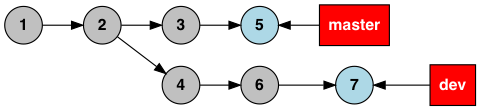
\includegraphics[width=.9\linewidth]{./images/diff-AB.png}
\caption{\label{fig:orgparagraph7}
Two commits in blue are compared in the output of both \texttt{git diff master dev} and \texttt{git diff master..dev} commands.}
\end{figure}
\begin{figure}[htb]
\centering
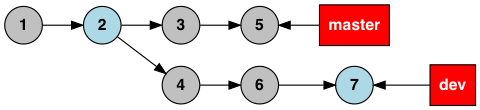
\includegraphics[width=.9\linewidth]{./images/diff-A___B.png}
\caption{\label{fig:orgparagraph8}
Two commits in blue are compared in the output of \texttt{git diff master...dev}. Note that commit 2 is the common ancestor of \texttt{master} and \texttt{dev} branches.}
\end{figure}

\subsection{\label{orgtarget8} Resolving Conflicts}
\label{sec:orgheadline19}
In this section, we will discuss scenarios in which conflicts occur, how Git represents merge conflicts, and how they can be resolved. Consider the following scenarios in which local branches are diverged from remote-tracking branches:
\begin{enumerate}
\item There exists no file modified in both local and remote commits. In this case, there will be no conflicts and merge will run smoothly; see Figure \ref{fig:orgparagraph9}-A.
\item There exist files modified in both local and remote commits, but there exists no overlapping lines in the modifications. In this case, there will be conflicts, but Git is expected to perform auto-merge without any issues; see Figure \ref{fig:orgparagraph9}-B.
\item There exists lines in some files modified in both local and remote commits. In this case, Git's auto-merge may perform a good job in resolving conflicts, however, manual conflict-resolution is expected; see Figure \ref{fig:orgparagraph9}-C.
\end{enumerate}
Scenario 3 is the only case we concern about in this section. We assume that there are overlapping changes in some parts of the files between the local and remote commits. Thus, when we pull from the remote repository, we should prepare for manual conflict resolution.

\begin{figure}[htb]
\centering
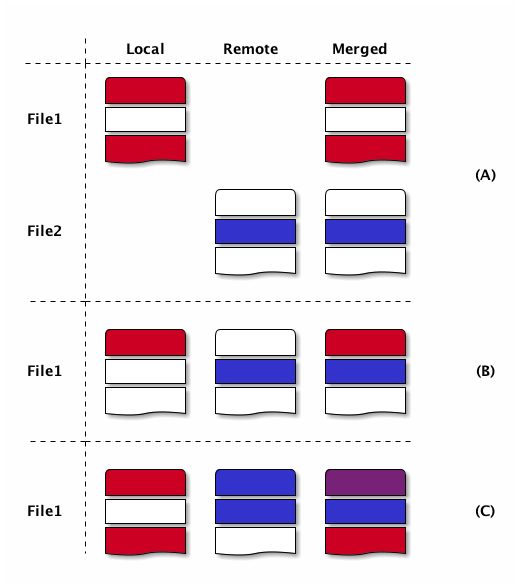
\includegraphics[width=.9\linewidth]{./images/resolving-conflicts.png}
\caption{\label{fig:orgparagraph9}
(A) No file has overlapping changes (automatic merge). (B) No line in any file has overlapping changes (automatic merge). (C) Lines in some files have overlapping changes (conflict: manual merge).}
\end{figure}

When we pull from the remote repository, Git may fail to resolve conflicts and request for manually resolving them. An example of \texttt{git pull} command may look like as follows:
\begin{verbatim}
$ git pull
 From https://github.com/eissana/test
  * [new branch]      master     -> origin/master
 Auto-merging README.md
 CONFLICT (content): Merge conflict in README.md
 Automatic merge failed; fix conflicts and then commit the result.
\end{verbatim}
The output explains a conflict in \texttt{README.md} file. A short status shows that there are unmerged changes:
\begin{verbatim}
$ git status -s
UU README.md
\end{verbatim}
Let us print the contents of the file:
\begin{verbatim}
$ cat README.md
# test
test.go implements a test program
<<<<<<< HEAD
add.go implements adding two numbers
=======
add.go implements addition
>>>>>>> 62840ed60259dca2bc90862672a663a9dcfe17b5
\end{verbatim}
To better visualize the position of the conflicting commits, let us print the log history:
\begin{verbatim}
$ git log --graph --decorate --oneline --all
 * 8a80440 (HEAD -> master) adding details regarding add.go into README.md
 | * 62840ed (origin/master) updated README.md with details of add.go
 |/
 * db2ac73 added add.go file
 * c9ffea7 added test.go
 * d17ef8a Added README.md
\end{verbatim}
Git represents conflicting lines using \texttt{<<<<<<< A ======= B >>>>>>>} notation. When merging, the format to remember is as follows:
\begin{verbatim}
<<<<<<< head of our changes (HEAD -> master)
our changes
=======
their changes
>>>>>>> head of their changes (origin/master)
\end{verbatim}
Note that when rebasing, the two parts are swapped. To continue with the merge, we have three options:
\begin{enumerate}
\item Accept our changes and overwrite theirs. This is performed by running \texttt{git checkout -{}-ours README.md} command.
\item Accept their changes and overwrite ours. This is performed by running \texttt{git checkout -{}-theirs README.md} command.
\item Reject both changes and introduce a new change. This is performed by manually opening the file in an editor of our choice and making changes.
\end{enumerate}
Once completed, we should stage our changes using \texttt{git add -A} and commit them with a proper commit message, before pushing them to the remote repository.

It is a good exercise to repeat above procedure with \texttt{git pull -{}-rebase} command. The notable difference is that the position of ``ours'' and ``theirs'' are swapped. Nevertheless, the same approach for resolving conflicts would work seamlessly.

\textbf{NOTE 1:} It is important to note that the merge-in-progress due to the conflict can be aborted at any time using \texttt{git merge -{}-abort} command. So, feel free to experiment resolving conflicts, as you can abort at anytime and start fresh.

\textbf{NOTE 2:} Sometimes, resolving conflicts are done in multiple steps. This happens when there are multiple conflicts, perhaps in multiple files. Once the first set of conflict resolution is completed, stage and commit the changes to move to the next step. Git may prompt us to resolve more conflicts. Once all sets of conflicts are completed, we exit the merging state.





\section{Summary}
\label{sec:orgheadline21}
This blog post aimed at presenting the minimal information you need to know to significantly boost your productivity with Git in managing repositories and versioning. In particular, we discussed the advantages of using a distributed version control system (DVCS), like Git, over a centralized VCS (CVCS), like Subversion. Then, we went through some details of configuring our environment to easily use Git's command-line tools. Such a configuration is important for performing all Git operations at ease.

We also introduced some Git notations, such as ancestry references and commit ranges, and saw an example of a commits graph. Then, we explained a typical Git workflow with interactions among a working Git directory, a local repository, and a remote repository. All such interactions can be carried out using Git's command-line tools.

Finally, we went through the most frequently used Git-commands to get the work done, including staging, committing, and pushing changes to a remote repository as well as branching, merging, rebasing, and stashing. The difference between merging and rebasing can be a source of confusion for novices, so we dedicated a section to provide more details and clear possible confusions. Both merging and rebasing may require manual conflict resolution. We discussed when conflicts might arise and how to resolve them in a separate dedicated section.

To obtain a complete picture of all historical changes in the repository, we showed how to use some of the Git's tools to inspect history of commits and visualize the position of branches and commits graph.

Most advanced topics, such as submodules, rewriting commits history, dealing with multiple work-trees, administrative tools such as \texttt{git fsck} and many more, are not covered in this blog post. To learn more about these advanced features and tools, one may consult Pro Git, which is freely available.
\end{document}